% Skip over this boring header down a bit
%%%%%%%%%%%%%%%%%%%%%%%%%%%%%%%%%%%%%%%%%%%%%%%%
\documentclass[usenames,twocolumn,dvipsnames,10pt,a4wide]{article} 
\usepackage[a4paper, total={8in, 10in}]{geometry}
% Add option 'aspectratio=169' for 16:9 widescreen 
% Add option  'handout' to ignore animations
% If you have a smaller amount of text, feel free to also try '11pt'! / Jesper

\usepackage[utf8]{inputenc}
\usepackage{verbatim}
\usepackage{minted}
\usemintedstyle{vs}
\usepackage{graphicx}
\usepackage{wrapfig}
\usepackage[document]{ragged2e}

\usepackage[shortlabels]{enumitem}

%%% Bibliography
\usepackage[style=authoryear,backend=biber]{biblatex}
\addbibresource{bibliography.bib}

\DeclareNameAlias{author}{given-family}

%%% Suppress biblatex annoying warning
\usepackage{silence}
\WarningFilter{biblatex}{Patching footnotes failed}

%%% Some useful commands
% pdf-friendly newline in links
\newcommand{\pdfnewline}{\texorpdfstring{\newline}{ }} 
% Fill the vertical space in a slide (to put text at the bottom)
\newcommand{\framefill}{\vskip0pt plus 1filll}


%%%%%%%%%%%%%%%%%%%%%%%%%%%%%%%%%%%%%%%%%%%%%%%%%%%%%%%%%%%%%%%%%%%%%%%%%%%%%%%%%%%%%
\title{Rust \#3: Collections, Iterators, and Traits}

\begin{document}

\maketitle

%\tableofcontents

\section{Collections in Rust}
	Rust's standard library implements some of
	the most common collections:
\begin{itemize}[label=$\bullet$]
	\item \textbf{Sequences}: String, Vec, VecDeque, LinkedList
	\item \textbf{Maps}: HashMap, BTreeMap
	\item \textbf{Sets}: HashSet, BTreeSet
	\item \textbf{Misc}: BinaryHeap
\end{itemize}
	In most cases, you are going to be fine with
	using just String, Vec, 
	HashMap, HashSet.


\subsection{Collections}
	\subsubsection{String}
	Strings are dynamic (heap-allocated) UTF-8 collections!
	\inputminted[fontsize=\normalsize]{rust}{code/string.rs}


\subsection{Collections}
	\subsubsection{String}
	\inputminted[fontsize=\normalsize]{rust}{code/string1.rs}


\subsection{Collections}
	\subsubsection{String}
	\inputminted[fontsize=\normalsize]{rust}{code/string2.rs}


\subsection{Collections}
	\subsubsection{String}
	\inputminted[fontsize=\normalsize]{rust}{code/string3.rs}


\subsection{Collections}
	\subsubsection{Vector}
	Vectors are your typical growable generic containers:
	\inputminted[fontsize=\normalsize]{rust}{code/vector.rs}


\subsection{Collections}
	\subsubsection{Vector}
	\inputminted[fontsize=\normalsize]{rust}{code/vector1.rs}


\subsection{Collections}
	\subsubsection{HashMap}
	HashMap is a 'dictionary' type that's generic over <K, V>:
	\inputminted[fontsize=\normalsize]{rust}{code/hashmap.rs}


\subsection{Collections}
	\subsubsection{HashMap}
	\inputminted[fontsize=\normalsize]{rust}{code/hashmap1.rs}


\subsection{Collections}
	\subsubsection{HashMap}
	\inputminted[fontsize=\normalsize]{rust}{code/hashmap2.rs}


\subsection{Collections}
	\subsubsection{HashSet}
	HashSet is a set that's generic over <T>:
	\inputminted[fontsize=\normalsize]{rust}{code/hashset.rs}


\subsection{Collections}
	\subsubsection{HashSet}
	\inputminted[fontsize=\normalsize]{rust}{code/hashset1.rs}



\section{Generics and Traits}

\subsection{Generics}
	\subsubsection{General}
	Generics are a common way to generalize types and
	functionalities. This can reduce code duplication and
	allow for different and user-defined types to be
	used with generic functions.


\subsection{Generics}
	\subsubsection{Generic structs and enums}
	We've already seen a few examples of generic types
	in Rust (as opposed to concrete types): 
	\inputminted[fontsize=\normalsize]{rust}{code/generics1.rs}


\subsection{Generics}
	\subsubsection{Generic structs and enums}
	Let's write one of these ourselves:
	\inputminted[fontsize=\normalsize]{rust}{code/generics2.rs}


\subsection{Generics}
	\subsubsection{Generic structs and enums}
	We can also be more specific with impl blocks:
	\inputminted[fontsize=\normalsize]{rust}{code/generics3.rs}


\subsection{Generics}
	\subsubsection{Functions}
	In Rust, generics can be used in a lot of cases,
	let's first look at generic functions.
	Let's imagine we have two functions that are
	basically the same except for parameter types:
	\inputminted[fontsize=\normalsize]{rust}{code/generics4.rs}


\subsection{Generics}
	\subsubsection{Functions}
	Let's rewrite these functions into a generic function:
	\inputminted[fontsize=\normalsize]{rust}{code/generics5.rs}
	This doesn't compile though...


\subsection{Traits}
	\subsubsection{General}
	Rust, at compile-time, needs to be sure that you
	won't be able to call these functions with a type
	that won't have the needed functionality.
	Rust has a concept that allows to tell the compiler
	about type's functionality, and to share that
	functionality between several types - traits.
	

\subsection{Traits}
	\subsubsection{General}
	What's the type functionality? Basically - just the
	methods we can call on that type, and traits
	allow us to group those methods in specific sets.
	Let's imagine we have several possible types of
	students - kindergarten, school and university
	students. We want to be able to get a report on
	them - with their names, grades etc.


\subsection{Traits}
	\subsubsection{Example}
	We define an 'interface' of our shared functionality
	with method signatures without any implementation.
	We can also provide default functionality for a trait:
	\inputminted[fontsize=\normalsize]{rust}{code/traits1.rs}


\subsection{Traits}
	\subsubsection{Example}
	Let's implement this trait for one of our student types:
	\inputminted[fontsize=\normalsize]{rust}{code/traits2.rs}


\subsection{Traits}
	\subsubsection{Traits as parameters}
	When we want to be sure that the type we take as a parameter
	has the needed functionality, we can use the impl Trait syntax:
	\inputminted[fontsize=\normalsize]{rust}{code/traits3.rs}


\subsection{Traits}
	\subsubsection{Traits as parameters}
	We can also specify having multiple traits
	implemented as a requirement:
	\inputminted[fontsize=\normalsize]{rust}{code/traits4.rs}


\subsection{Traits}
	\subsubsection{Traits as parameters}
	If your function is generic over several types with
	different trait bounds, it's better to use where syntax:	
	\inputminted[fontsize=\normalsize]{rust}{code/traits5.rs}


\subsection{Generics and Traits}
	\subsubsection{Bounds}
	Let's return to an earlier example of a generic function:
	\inputminted[fontsize=\normalsize]{rust}{code/generics5.rs}


\subsection{Generics and Traits}
	\subsubsection{Bounds}
	Why didn't it compile? Well, the compiler is actually quite helpful:
	\inputminted[fontsize=\normalsize]{rust}{code/generics6.rs}


\subsection{Generics and Traits}
	\subsubsection{Bounds}
	Let's look at that std::ops::Add:
	\inputminted[fontsize=\normalsize]{rust}{code/generics7.rs}


\subsection{Generics and Traits}
	\subsubsection{Bounds}
	Let's add a bound on our generic function:
	\inputminted[fontsize=\normalsize]{rust}{code/generics8.rs}
	But this doesn't compile, again...


\subsection{Generics and Traits}
	\subsubsection{Bounds}
	Once again, Rust compiler saving our souls:
	\inputminted[fontsize=\normalsize]{rust}{code/generics9.rs}


\subsection{Generics and Traits}
	\subsubsection{Bounds}
	Alright, let's restrict it even further, now also
	considering that we don't want to borrow our
	arguments, we want to copy them:
	\inputminted[fontsize=\normalsize]{rust}{code/generics10.rs}


\subsection{Generics and Traits}
	\subsubsection{std Traits}
	The standard library implements a lot of traits
	which allow it to reason about the functionality
	that certain types might have. The Copy one
	we used	is a good example.
	\inputminted[fontsize=\normalsize]{rust}{code/traits6.rs}
	This allows the Rust compiler to understand whether
	to move the object out or to copy it. 	


\subsection{Generics and Traits}
	\subsubsection{std Traits}
	If the type implements a Copy trait, it's usually just
	called Copy. For example, i32 is Copy, because it
	implements the trait and won't move out:
	\inputminted[fontsize=\normalsize]{rust}{code/traits7.rs}


\subsection{Generics and Traits}
	\subsubsection{std Traits}
	The standard library provides a lot of traits with default
	implementations which you can derive, among them:
	\begin{itemize}[label=$\bullet$]
		\item \textbf{Debug} - Debug formatting using :?
		\item \textbf{PartialEq} and \textbf{Eq} - For $!=$ and $==$ implementations
		\item \textbf{PartialOrd} and \textbf{Ord} - For orderings using $<, >, <=, >=$
		\item \textbf{Hash} - Allows to map an instance to a value
	\end{itemize}
	There are also 'marker' traits without any implementations,
	but they are beyond the scope of this lecture.



\section{Lifetimes}
\subsection{Lifetimes}
	We've already talked about lifetimes a little, but so far
	we've mainly relied on the compiler to figure out lifetimes
	for us. Sometimes it's impossible for the compiler to
	reason about lifetimes, and we are forced to help it out.
	This is where generic lifetimes come in. Yes, Rust has a lot
	of generic stuff - your functions can operate on generic
	types, 'generic' trait-implementing types and lifetimes.


\subsection{Lifetimes}
	Let's remind ourselves how Rust compiler
	reasons about lifetimes:
	\inputminted[fontsize=\normalsize]{rust}{code/lifetimes1.rs}


\subsection{Lifetimes}
	And now in the case of a simple function:
	\inputminted[fontsize=\normalsize]{rust}{code/lifetimes2.rs}


\subsection{Lifetimes}
	If the references do not contain explicit lifetime annotations,
	they are instead called implicit. We can write simple functions
	without explicitly annotating lifetimes of our parameters (just
	how we can omit types sometimes), and the function will be
	figured out by the compiler like this:
	\inputminted[fontsize=\normalsize]{rust}{code/lifetimes3.rs}


\subsection{Lifetimes}
	Generally, when it is possible, Rust compiler does not need
	our help and is able to figure out the lifetimes on its own.
	It uses several rules for figuring out the lifetimes for functions:
	\begin{itemize}[label=$\bullet$]
		\item Each parameter that is a reference gets its own lifetime
		\item If there is one input lifetime, this lifetime is assigned
			to the return value
		\item If there are several input lifetimes, but one is self,
			its lifetime is assigned to the return value
	\end{itemize}


\subsection{Lifetimes}
	Let's try to apply these rules in a more complex case:
	\inputminted[fontsize=\normalsize]{rust}{code/lifetimes4.rs}


\subsection{Lifetimes}
	Rust compiler is not able to figure out the lifetime
	of the returned reference with these rules:
	\inputminted[fontsize=\normalsize]{rust}{code/lifetimes5.rs}


\subsection{Lifetimes}
	It will complain and try help us:
	\inputminted[fontsize=\normalsize]{rust}{code/lifetimes6.rs}


\subsection{Lifetimes}
	Let's introduce a single named lifetime parameter:
	\inputminted[fontsize=\normalsize]{rust}{code/lifetimes7.rs}


\subsection{Lifetimes}
	One special lifetime in Rust is 'static:
	\inputminted[fontsize=\normalsize]{rust}{code/lifetimes8.rs}
	It means that the reference will live for the entire
	duration of the program (indeed, string literals
	are just embedded into the program binary).
	The compiler will often suggest you use this
	lifetime as an annotation, but you should only
	use it when it makes sense!


\subsection{Lifetimes}
	Rust functions can often get pretty messy when you use
	generic types, lifetimes and trait bounds:
	\inputminted[fontsize=\normalsize]{rust}{code/lifetimes9.rs}


\section{Iterators}

\subsection{Iterators}
TODO: talk about iterators, closures, functional programming etc.
	

 

%\subsection{Resources}
	%\Large
	%\begin{figure}[c]
		%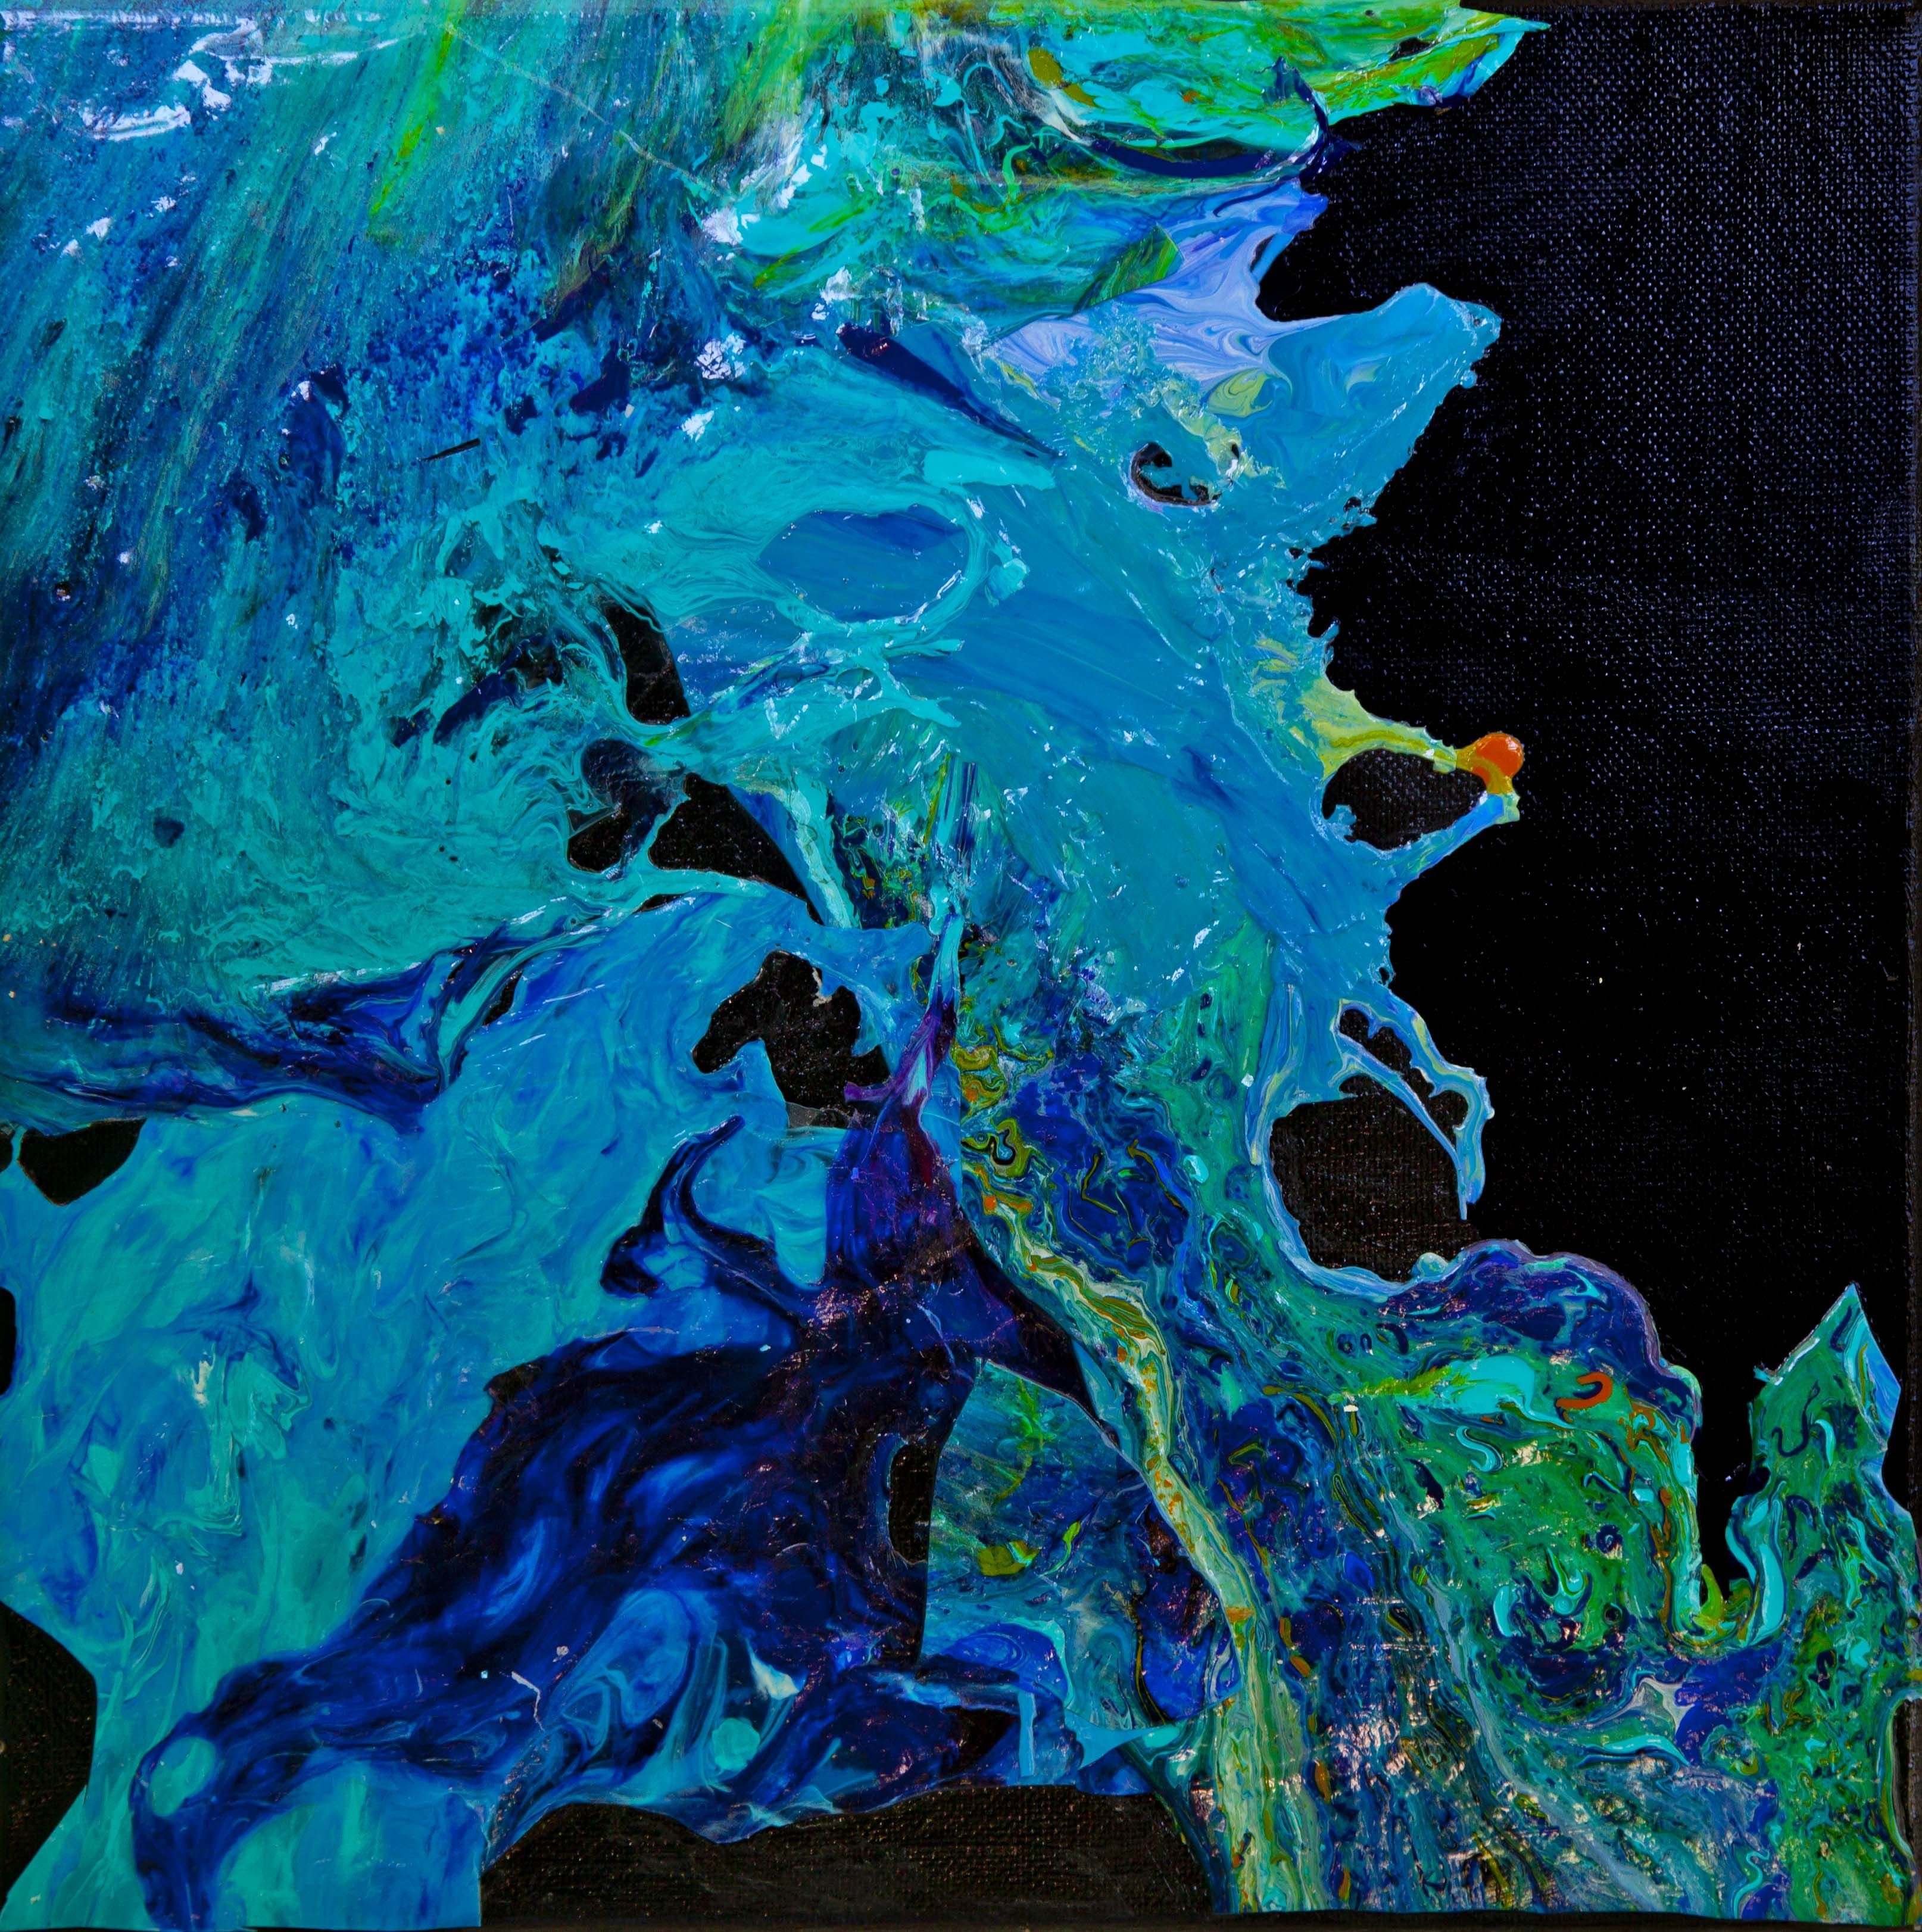
\includegraphics[width=1\linewidth]{graphics/1.jpg}
	%\end{figure}
%

 \end{document}
